\begin{theo}[De wet van de universele zwaartekracht]{De wet van de universele zwaartekracht}

Elk deeltje in het heelal trekt elk ander deeltje aan met een kracht die recht evenredig is met het product van hun massa’s en omgekeerd evenredig met het kwadraat van de onderlinge afstand, in formulevorm:
 
 \begin{equation*}
     F_g = G\dfrac{m_1m_2}{r^2} \text{ met } G = 6.673 \times 10^{-11} \dfrac{Nm^2}{{kg}^2}
 \end{equation*}
 
\noindent We weten natuurlijk al uit voorgaande hoofdstukken wat de formule voor de zwaartekracht is nabij het aardoppervlak is, maar hoe komen we hieraan?

\begin{equation*}
    F_a = G\dfrac{mM_a}{(R_a+h)^2} \approx G\dfrac{mM_a}{r_a^2} = mG\dfrac{M_a}{r_a^2} \Rightarrow F_a = mg \text{ met } g = G\dfrac{M_a}{r_a^2}
\end{equation*}

% \noindent Als we nu stellen dat $ g = G\dfrac{M_a}{r_a^2} $, dan volgt:

% \begin{equation*}
%     F_a = mg
% \end{equation*}

\noindent \textbf{Let op:} De formule spreekt over twee puntmassas! Een macroscopisch voorwerp is een som (\textbf{integraal!}) over een zeer grote verzameling puntmassas, dus hoe moeten we het hier berekenen?
\begin{itemize}
    \item \textbf{Symmetrische bol:} alsof alle massa in het middelpunt zit
    \item \textbf{Symmetrische schil:} alsof alle massa in het middelpunt zit, én enkel kracht op massa buiten de schil
\end{itemize}

\end{theo}

\begin{app}[Satellieten]{Satellieten}

    Satellieten voeren een ECB uit rond de aarde. Er moet dus een centripetale kracht zijn die een satelliet op zijn baan houdt. Als we de tweede wet van newton zouden gebruiken vinden we in de radiale richting het volgende: 
    
    \begin{equation*}
        \sum F_R = G\dfrac{mM_a}{r_a^2} = m \dfrac{v^2}{r_a} \ met \ r_a = R_A + h_s
    \end{equation*}
    
    
    \noindent Hieruit volgt dat de tangentiêle snelheid, die de satteliet op zijn baan houdt, gelijk is aan het volgende:
    
    \begin{equation*}
        v = \sqrt{\dfrac{GM_a}{r}} = \sqrt{\dfrac{GM_a}{R_A + h_s}}
    \end{equation*}
    
    % \noindent \textbf{Opmerking:} een lagere/hogere baan heeft dus een hogere/lagere snelheid nodig

\end{app}

\begin{theo}[Gravitatieveld]{Gravitatieveld}
    
    % Volgens het veldconcept omringt een gravitatieveld elk voorwerp met massa en dit veld doordringt de hele ruimte. Een tweede voorwerp op een bepaalde plaats in de buurt van het eerste voorwerp ondervindt een kracht vanwege het daar aanwezige zwaartekrachtsveld. We kunnen het gravitatieveld definiëren als de gravitatiekracht per massa-eenheid op een willekeurig punt in de ruimte.
    
    Als we het gravitatieveld op een willekeurig punt willen meten, plaatsen we een kleine testmassa op dat punt en meten we de kracht die erop wordt uitgeoefend (waarbij we ervoor zorgen dat er alleen gravitatiekrachten werken). Dan is het gravitatieveld op dat singulier punt gedefinieerd als: 
    
    \begin{equation*}
        \Vec{g} = \dfrac{\Vec{F}}{m} = \dfrac{1}{m}G\dfrac{mM}{r^2}\hat{r} = -\dfrac{GM}{r^2}\hat{r} 
    \end{equation*}

\end{theo}

% \begin{ex}[Voorbeeld: Geostationaire satelliet]{Geostationaire satelliet}

%     \centering
%     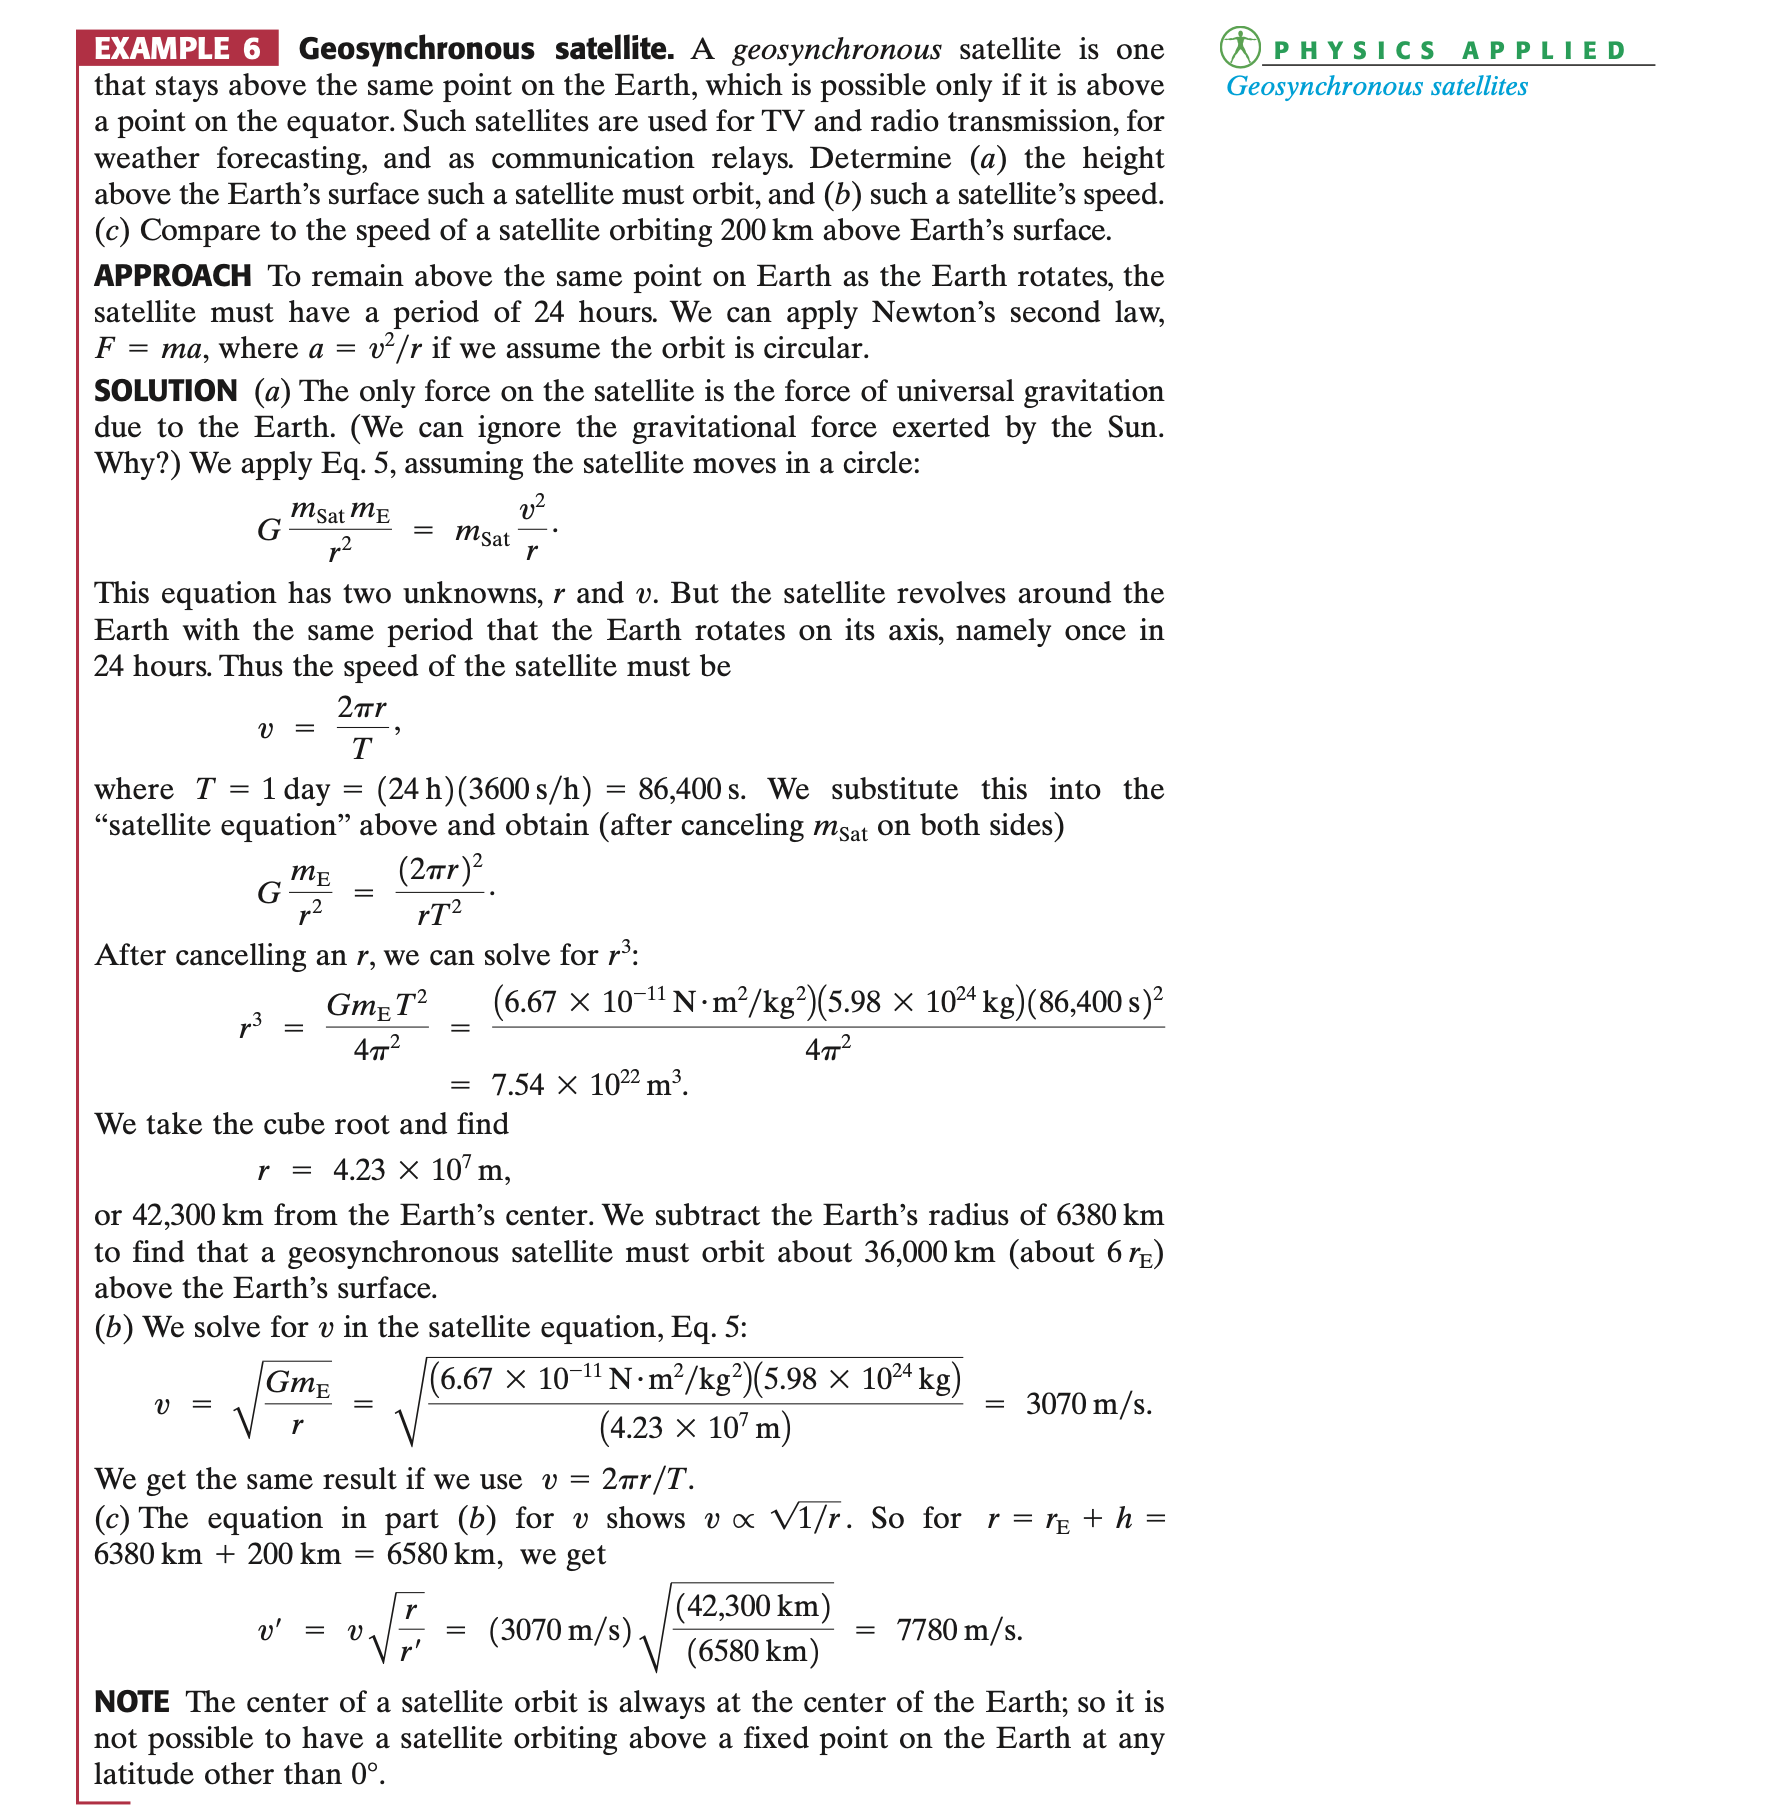
\includegraphics[scale = 0.5]{Examples/Dynamica/6.6.png}
    
% \end{ex}
